\chapter{Background}
\label{chp:background}
This chapter presents the background and literature on locomotion mode recognition systems for prostheses. The chapter contains seven sections. Firstly background around human gait and prostheses are presented in Sections \ref{sec:background-gait} and \ref{sec:background-Prosthesis}. Following this, Section \ref{sec:background-sensors} reviews wearable sensors used for gait analysis. Sections \ref{sec:background-machine-learning} and \ref{sec:background-ml-lmr} contain an introduction to machine learning and its applications for Locomotion Mode Recognition. Finally, concluding remarks about areas of research interest are presented in Section \ref{sec:background-conclusion}.

%---------------------------------------------%
\section{Biomechanics of Gait}
\label{sec:background-gait}
Human locomotion involves the smooth advancement of the body through space with the least mechanical and physiological energy expenditure. While the primary goal of walking is forward motion, the mechanism that achieves it is based on the need to maintain a symmetrical and low amplitude displacement of the body's \acrshort{com} in both vertical and lateral directions. Low displacement conserves both kinetic and potential energy and is the principle of biological conservation of energy.\cite{Waters1999}

Gait is a highly individualistic personal trait with many factors that affecting it\cite{Horst2019}. A performant gait is a coherent highly energy-efficient mechanism for forward propulsion of the body. It naturally adapted to different environmental conditions and disturbances to achieve high level of stability throughout the gait cycle\cite{Shah2020, Mummolo2013}. With regards to lower-limb prosthetic the mechanics of locomotion are of most interest. Within this section the terminology that will be used to with reference to the human gait and the high level biomechanics of locomotion are presented.

Different ambulation modes require fundamentally different control sequences for operating powered prosthetic limbs\cite{Hargrove2015}. There are a large number of possible locomotive activities depending on the environment and movement speed. In the study of activity recognition level-ground walking, ramp ascent, ramp descent, stair ascent, and stair descent are the most commonly studied\cite{Hargrove2013, Young2013, Simon2013, Godiyal2018a, Rai2019, Su2019, Labarriere2020, Srisuwan2021, Bruinsma2021} and cover the most basic locomotion activities used for forward motion\cite{Ebner2020}. Labarri\`ere et al.~identified these as the most commonly investigated as they require no equipment or skill to perform\cite{Labarriere2020}.

\subsection{Gait Terminology}
A complete gait cycle is the basic unit of gait analysis. A cycle, by convention, begins when one foot comes into contact with the ground, \acrfull{ic}, and is complete when the same foot contacts the ground again. Another name for \acrshort{ic} is \acrfull{hs}, as the heel is the most common initial point of contact. Conversely, the point at which the foot leaves the ground is \acrfull{to}. The name arises as the toe is always the last point of contact with the ground.\cite{Novacheck1998, Shah2020}

The gait cycle can be further sub-divided into two phases. The distinct phases, stance and swing, are physically indicated by the foot's contact with the ground. Stance occurs when the foot is in contact with the ground, and swing occurs when the foot is off the ground. \acrshort{hs} marks the transition from swing to stance and \acrshort{to} stance to swing. When considering both limbs, there are additional descriptors. These include single support when only one foot is in contact with the ground and double support when both feet are in contact with the ground. Figure \ref{fig:background_gait_cycle} illustrates a complete gait cycle and the key events.\cite{Novacheck1998, Shah2020}

% Picture of gait cycle indicating key events
\begin{figure}[!hbt]
    \centering
    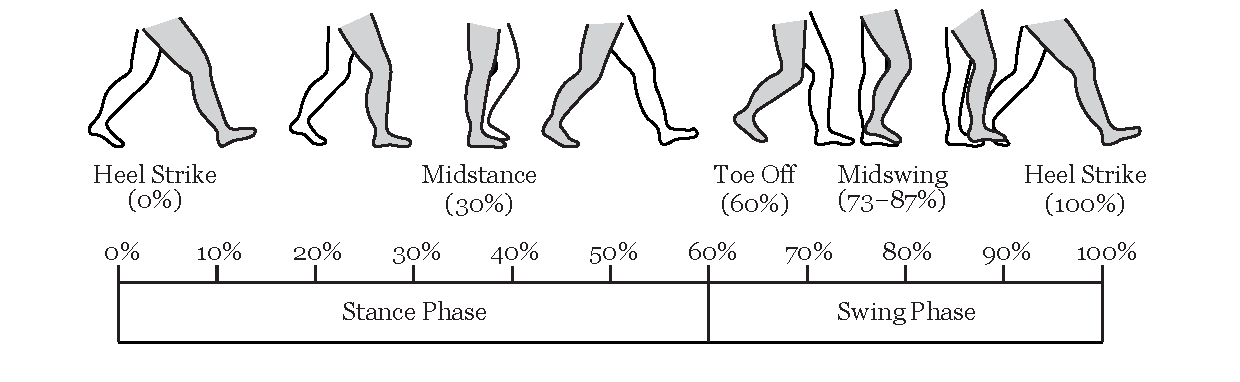
\includegraphics[width=\textwidth]{content/4-LSTM_Behaviour/Gait_Cycle.pdf}
    \caption[Human Gait Cycle during level walking]{Human Gait Cycle during level walking. The percentage timings of the gait events are approximate; they vary depending on the individual and environment.\cite{Sherratt2021}}
    \label{fig:background_gait_cycle}
\end{figure}

Movements of the human body mainly occur in three planes: sagittal, frontal/mediolateral and horizontal/transverse. The plane's intersections occur either at a joint centre or the body's \acrfull{com}. The sagittal plane is the vertical plane passing from the rear (posterior) to the front (anterior), dividing the body left and right. The mediolateral plane passes from left to right, dividing the body into posterior and anterior halves. The transverse plane divides the body into the top (superior) and bottom (inferior) halves.\cite{Bartlett2007} Figure \ref{fig:background_planes_of_the_body} shows an illustration of the three planes

% Image of different planes of human motion
\begin{figure}[!hbt]
    \centering
    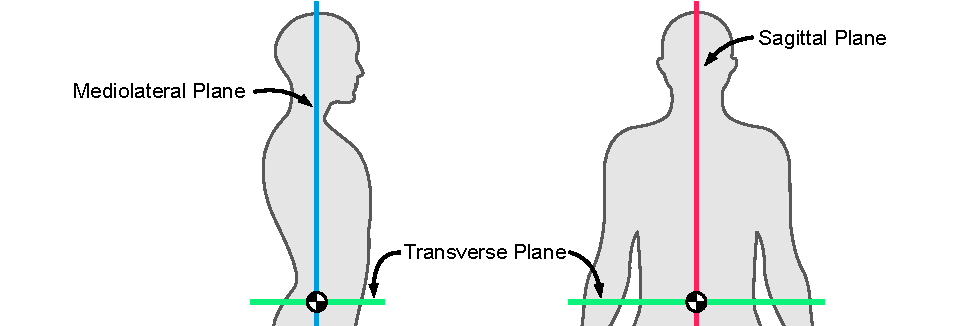
\includegraphics[width=0.9\textwidth]{content/2-Background/body_planes.pdf}
    \caption[Bio-mechanical planes of the body]{Bio-mechanical planes of the body. The sagittal plane is the vertical plane dividing left and right body halves. The mediolateral plane divides the body into front and rear halves. Finally, the transverse plane divides the body into the top and bottom halves.}
    \label{fig:background_planes_of_the_body}
\end{figure}

The primary movement of the ankle occurs in the sagittal plane; these are the raising and lowering of the foot. The two motions are plantar-flexion, moving the foot downwards, and dorsiflexion, lifting the foot upwards.\cite{Bartlett2007} Figure \ref{fig:background_plantar_dorsi_flexion} show a visual of the ankle movement.  Plantar-flexion happens towards the end of the stance phase when the foot pushes off the ground. Dorsiflexion occurs during the early swing phase to provide enough toe clearance as the foot passes under the body.\cite{Whittle2012}

\begin{figure}[!hbt]
    \centering
    
\includegraphics[width=\textwidth]{content/2-Background/Ankle_Flexion.pdf}
    \caption[Sagittal plane motions of the ankle]{Sagittal plane motions of the ankle. Plantar flexion is the lowering of the foot; dorsiflexion is the raising of the foot.}
    \label{fig:background_plantar_dorsi_flexion}
\end{figure}

There are many different metrics for quantifying gait. These vary from easily measurable values such as step rates and distances to more involved metrics such as energy expenditure and efficiency.\cite{Ramakrishnan2019, Coutts1999}. Measurements of energy expenditure are not possible directly. Energy expenditure must be is calculated indirectly, this is commonly done through measurement of the volume of oxygen consumed and carbon-dioxide produced. The equipment required for measurements restrict energy measurements to a lab environment.\cite{Waters1999}

%---------------------------------------------
\subsection{Variation with Locomotive Activity}
The previous section described the pattern of gait that occurs during a level walking locomotion. The human gait cycle can efficiently adapt to different terrain and obstacles. Changes in the locomotive activity require a change in gait actions to accomplish the movement\cite{Hargrove2015}. Additional muscle actions are required to raise and lower the \acrshort{com} during these actions\cite{Franz2012a}.

This section presents bio mechanical difference between five different locomotive movements, Walking, \acrfull{sa}, \acrfull{sd}, \acrfull{ra}, \acrfull{rd}. Ramps are considered any surface with a slope sufficiently steep so that a change in locomotive action is required. For each activity, there is a description of the differences in human gait compared to walking.

\subsubsection{Stair Ascent}
During \acrshort{sa}, the \acrshort{com} must move upwards, requiring net positive work; this requires more significant muscle activity. \acrshort{sa} can be divided into three phases: weight acceptance, pull-up and forward continuation. The knee dominates during weight acceptance and pull-up with support from the hip and ankle. While, during forward continuation, the ankle generates a large amount of energy resulting in an upwards motion of the \acrshort{com}. The ankle angle differs from a horizontal walk, mainly at the late swing phase and early stance. While lifting the foot to the next tread, the edge is avoided by a small dorsiflexion and moving the knee backwards.\cite{Svensson2007} The changes in gait cycle are illustrated in Figure \ref{fig:stair-ascent-gait-cycle}.

\begin{figure}[!hbt]
    \centering
    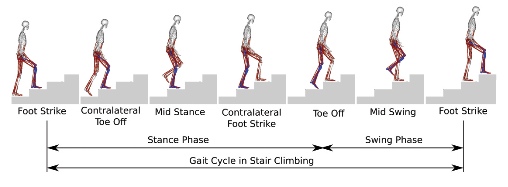
\includegraphics[width=0.9\textwidth]{content/2-Background/sa_gait_cycle.pdf}
    \caption[Stair ascent gait cycle]{Stair ascent gait cycle\cite{Cheung2020}}
    \label{fig:stair-ascent-gait-cycle}
\end{figure}

\subsubsection{Stair Descent}
During \acrshort{sd}, the ankle angle differs from horizontal in the swing phase when moving the limbs down. The change in ankle angle is most notable as a dorsiflexion action to reaching the toe downwards. The change in ankle angle results in the toe being the point of \acrshort{ic}. Energy is transferred from the ankle into the knee at \acrshort{ic}. Due to the downwards, \acrshort{com} motion reflects in a smaller force at push-off. There is also less muscle activity for vertical movements due to the smaller stride length.\cite{Svensson2007} The changes in gait cycle are illustrated in Figure \ref{fig:stair-descent-gait-cycle}.

\begin{figure}[!hbt]
    \centering
    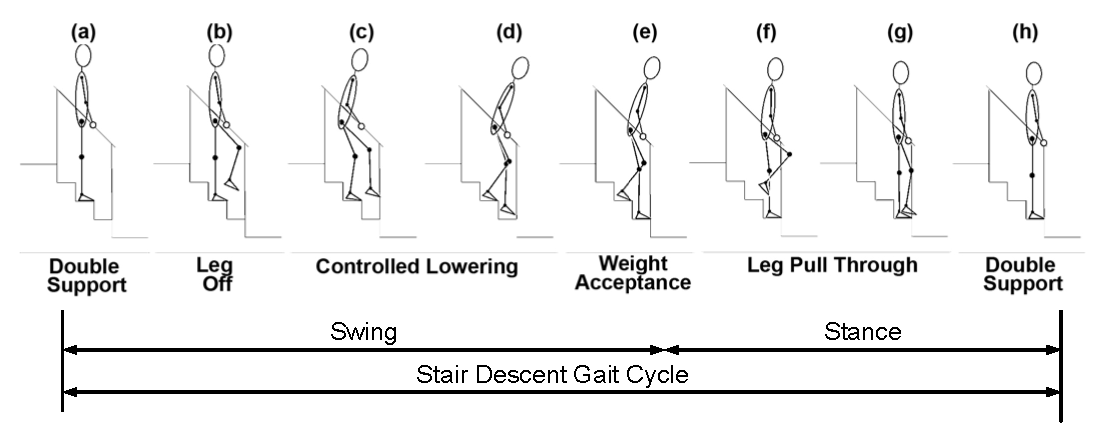
\includegraphics[width=0.9\textwidth]{content/2-Background/sd_gait_cycle.pdf}
    \caption[Stair descent gait cycle]{Stair descent gait cycle\cite{Bulea2014}}
    \label{fig:stair-descent-gait-cycle}
\end{figure}

\subsubsection{Ramp Ascent}
As with \acrshort{sa}, \acrshort{ra} requires additional energy expenditure to move the \acrshort{com} upwards\cite{Franz2012a}. Walking uphill can take three times as much energy as walking on flat ground\cite{Matsumoto2017}. Gait parameters also vary with the slope of the surface\cite{Kimel-Naor2017}. Knee flexion and ankle dorsiflexion increases at heel strike as the foot aligns with the surface. These changes in gait require an increased range of motion and additional muscle power generation.\cite{McIntosh2006}

\subsubsection{Ramp Descent}
For moderate slopes, \acrshort{rd} is similar to level walking. However, the lowering of the \acrshort{com} requires additional energy to be absorbed\cite{Franz2012a}. Walking downhill takes only half as much energy as walking on the level ground\cite{Matsumoto2017}. As with \acrshort{ra}, the gait adjusts to the slope.

The above describes the steady-state motions during typical locomotive activities. The human gait can also smoothly transition between different locomotive modes and handle perturbations and disturbances.\cite{Li2019}

\subsection{Gait variations between Amputee and Non-Amputee}
Amputees suffer from a wide range of gait abnormalities when compared to non-amputees. These occur both due to mechanical constraints of a prosthesis and compensatory actions due to the functional loss of muscles~\cite{Rabuffetti2005, Silverman2008}. These adaptations are individual and unique to the amputee and their particular amputation~\cite{Lechler2018, Kovac2009}. General trends in the adaptation may be drawn, such as asymmetrical gait, slower walking speed, and higher energy demands\cite{Burkett2004}.

Amputee gait is significantly more asymmetrical compared to that of a non-amputee, with amputees relying more heavily on their intact limb~\cite{Bateni2002, Varrecchia2019}. Asymmetry is seen in many gait features, including stance and swing periods and hip, knee and ankle joint moments\cite{Adamczyk2015, Harandi2020}. A common explanation for this is the reduced push-off capacity of the prosthetic leg, but it may also be due to discomfort of the prosthetic and other compensatory mechanisms\cite{Hak2014}.

Energy expenditure measurement have proven to be a reliable method of quantitatively assessing the penalties imposed by gait disability~\cite{Waters1999}. Studies have shown that trans-tibial amputees using passive prosthesis use 10-40\% more energy to walk at the same speed when compared to their non-amputee peers~\cite{McDonald2018, Herr2012}, with trans-femoral amputees requiring more than 70\%~\cite{Stewart2008}. This additional energy expenditure dramatically impedes ambulation. Amputees are half as active as their non-amputee peers and prefer 30-40\% slower walking speeds~\cite{Bussmann2008, Piazza2017, Lin2014, Au2009}. The loss of significant power generating muscles after amputation also leads to a marked asymmetry in gait between limbs~\cite{Button2010}.

Amputee subjects walk at a 29\% lower comfortable speed than a non-amputee~\cite{ Jaegers1995, Boonstra1993}. They also walk with a larger stride width than normal subjects~\cite{Jaegers1995}. To achieve higher walking speeds amputees prefer to adjust their stride length rather than with their step rate~\cite{Jaegers1995, Rabuffetti2005}.

Insufficient mid swing toe clearance of a prosthetic foot is a well-recognised inadequacy for lower limb prosthesis user due to inability to adequately dorsi-flex the ankle. The lack of toe clearance results in an increased risk of tripping~\cite{Lechler2018}. Compensatory mechanisms are employed by the amputee to reduce tripping risk. A common mechanism is elevating the prosthetic hip during mid-swing referred to as Vaulting or hip-hiking. Elevation is achieved by employing an early heel rise of the intact limb.\cite{Drevelle2014, Lechler2018}. Hip-hiking increases the \acrshort{com} height during swing on the amputated limb when compared to a non-amputee. The increased \acrshort{com} reduces gait efficiency and the asymmetry of the gait can lead to injury.


Lower limb amputees spend more time in stance on their intact limb and less on their prosthetic limb~\cite{Nolan2003}. The double-limb-support phases of the intact and prosthetic side are unequal in most amputee subjects~\cite{Jaegers1995}. In particular the different characteristics of the prosthesis relative to the sound limb results in a longer swing time for the prosthesis~\cite{Burkett2004}. This asymmetry increased with walking speed~\cite{Nolan2003}.

An amputee also have an asymmetric \acrfull{grf}. Able-bodied subjects have less than 10\% force asymmetry during walking while unilateral amputees have up to 23\% force asymmetry depending on the type of prosthesis used~\cite{Nolan2003}. There is also a decreased \acrshort{grf} on prosthesis compared to a non-amputee\cite{Kovac2009}. Many lower limb amputees attempt to maximise the capacities of their intact limb to counteract the limitations of their prosthetic device explaining some of the \acrshort{grf} asymmetry\cite{Ochoa-Diaz2020}. 




%---------------------------------------------%
\section{Lower Limb Prosthesis}
\label{sec:background-Prosthesis}
A lower-limb amputation involves the removal of part, or multiple parts, of the lower limb. The practice of amputation for injury or disease is centuries old and likely first occurred in pre-historic times\cite{Kirkup2007}. The level of amputation can be either minor or major, depending on the amputation site. Major lower limb amputations occur above the ankle. The two most common major lower limb amputations are trans-femoral (above the knee) and trans-tibial(below the knee).

An artificial or prosthetic limb can replace an amputated extremity. The prosthesis aims to restore natural behaviour by emulating/augmenting the action of a missing limb.\cite{Tucker2015} The ability of a prosthesis to mimic the function and appearance of the lost limb can vary significantly.

The earliest known prostheses are recorded in Indian literature between 1500 to 800 b.c. although artificial limbs are probably much older than that\cite{Breakey1976}. Over the years, prostheses have gone from barely functional to sophisticated devices aiming to replicate lost functionality. Artificial limb design, fitting and manufacture has advanced considerably within the past 50 years and is now a burgeoning research field.\cite{Kirkup2007}

% Types of prosthetic
The current primary technologies for prosthetic legs are: \acrfull{esr}, hydraulics, semi-active and active devices\cite{Asif2021}. Figure \ref{Fig:CH2-prostheses_type} shows examples for each type.

\begin{figure}[!hbt]
    \centering
    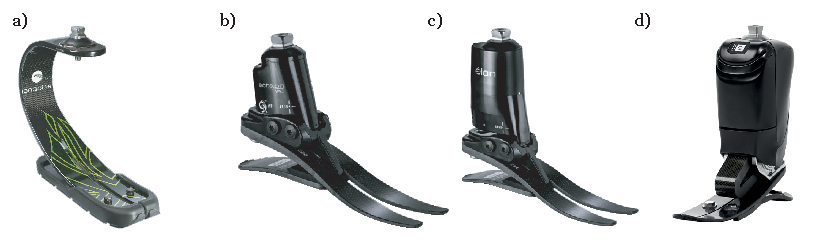
\includegraphics[width=\textwidth]{content/2-Background/ch2_prosthetic_device_types.pdf}
    \caption[Example prostheses types]{Example prostheses types: a) ESR (Blatchford BladeXT), b) Hydraulic (Blatchford EchelonVAC), c) Semi-active (Blatchford Elan), d) Active (Ottobock's biOM) (a-c)\cite{blatchford2018} (d)\cite{biom2018} }
    \label{Fig:CH2-prostheses_type}
\end{figure}

Each technology offers varying levels of assistance, with amputee suitability and preference informing selection. The most common form of prostheses is the \acrshort{esr} foot. During walking, an ESR prosthesis reduces energy expenditure by storing energy through spring compression during heel loading, releasing it during late stance to push-off.\cite{Asif2021}

Passive devices such as an \acrshort{esr} cannot provide the net positive mechanical power needed during many activities of daily living, such as ascending stairs or standing up from a seated position\cite{Simon2013}. To fully restore gait functionality, the prostheses must replace the lost power generating function of the amputated limb.

A powered active prosthetic device could provide the full power-output capabilities of the corresponding physiological joints. It could thus enable gait patterns resembling those of unaffected persons across various activities and terrain\cite{Tucker2015, Bhakta2020}. According to Au et al., The use of an active prosthetic can reduce metabolic energy usage by 14\% in trans-tibial amputees, even with a two-fold increase in prosthetic weight\cite{Au2009}.

Ottobock's BiOM EmPOWER active prosthetic ankle is currently the only active prosthetic device on the market.\cite{Nayak2020} The device is a spin-out from research undertaken by MIT in 2011.\cite{biom2018} Analysis of the EmPOWER ankle has shown a reduction in the metabolic cost of walking by 8\% and an increased walking velocity of 23\%\cite{Herr2012}.\ {\"O}ssur produces the Proprio Foot, a semi-active ankle that lifts the toe to increase ground clearance. The Proprio foot has also been integrated with their Rheo Knee to form a coordinated leg for trans-femoral amputees capable of stair descent.\cite{Ossur}

% ----------------------------------
\subsection{Control Requirements for Powered Prosthesis} % Introduce the problem
The human body represents a well-balanced walking machine that performs periodic, stable, and energy-efficient gait through highly sophisticated mechanics and control, which are not easy to replicate\cite{Mummolo2013}. The human nervous system uses different control strategies to adapt to individual locomotive activities\cite{Lay2007, Simon2013}. These adaptations occur automatically in a healthy gait cycle. A prosthetic controller must implement multiple control modes to replicate this lost functionality.

An active prostheses controller must implement several concurrent processes to control prostheses effectively. Tucker et al.~present a generalised hierarchical framework for structuring a prostheses controller. Hardware control forms the lowest level. The top-level controller implements a perception system to determine user intent or activity mode. Therefore, an accurate perception of the users' intended action is paramount\cite{Asif2021, Hernandez2021}. An intermediate level controller performs translation of intent to hardware state demands. An illustration of the hierarchical controller is provided in figure \ref{Fig:lit-rev-controller_framework}.\cite{Tucker2015}

\begin{figure}[!hbt]
    \centering
    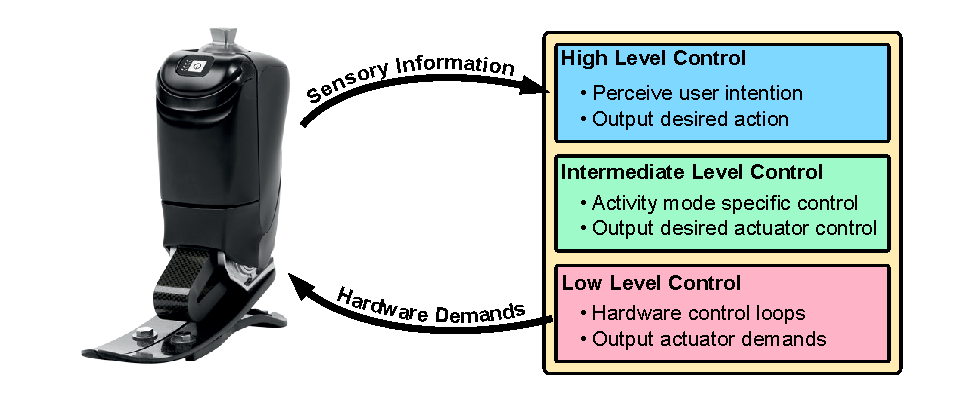
\includegraphics[width=\textwidth]{content/2-Background/control_hierarchy.pdf}
    \caption{Generalised control framework for active lower limb prostheses}
    \label{Fig:lit-rev-controller_framework}
\end{figure}

\subsubsection{High Level Controller}
As different activities require changes to gait pattern multiple mid-level controllers are required for each locomotive tasks; for example walking, standing still or stair descent. Selection of the appropriate mode is critical to performance of this controller as selection of the wrong mode will result in undesirable behaviour. The high level controller is responsible for the selection of the appropriate mid-level controller.\cite{Tucker2015}

There are many different forms of mode selection including manual user entry, heuristic threshold methods\cite{Varol2010, Kazemimoghadam2021, Rabe2021} and machine learning methods\cite{Li2022, Wang2019b}. All of these methods use sensors to interpret user intent and environment around them to make an appropriate mode selection.

\subsubsection{Mid Level Controller}
The mid controller is responsible for determining the demand physical state of the device throughout the gait cycle. The selection of demand state is driven by the which phase of the gait cycle the user is in, and the current activity mode. The demand states have the form of a position/velocity, torque or, impedance of different prosthetic components which are fed to the low level controller to enforce.\cite{Tucker2015}

Most mid-level controllers have a finite number of modes corresponding to a series of different activity sequences. Researchers are also investigating continuous or mode free controller to reduce the need for bespoke state machines per activity.\cite{Rai2019b, Bartlett2021}

Accurate determination of the current gait phase is critical to outputting appropriate demand signals. When done correctly this allows the prosthetic to provide a natural walking gait and to make the most use of any power generating/absorbing capacity
For example Yu et al.~presented a prosthetic ankle that could provided powered plantar-flexion. From the work it was identified that accuracy timing of the plantar-flexion was critical. Plantar-flexing  too early resulted in the ankle lifting the body upward instead of pushing the body forward. Powering the plantar-flexion too late resulted in a lack of support of the body weight, with the amputee in danger of stumbling.\cite{Yu2019}

Sup et al.~illustrated an example mid-level state machine as shown in Figure \ref{fig:mid-level-state-machine}. The selection of modes is achieved based on threshold for different sensor inputs being reached. For example mode one begins after mode four when the measure ankle loading exceeds a manually set threshold. The state machine moves to mode two when the ankle angle exceed another threshold value.\cite{Sup2008b}

\begin{figure}[!hbt]
    \centering
    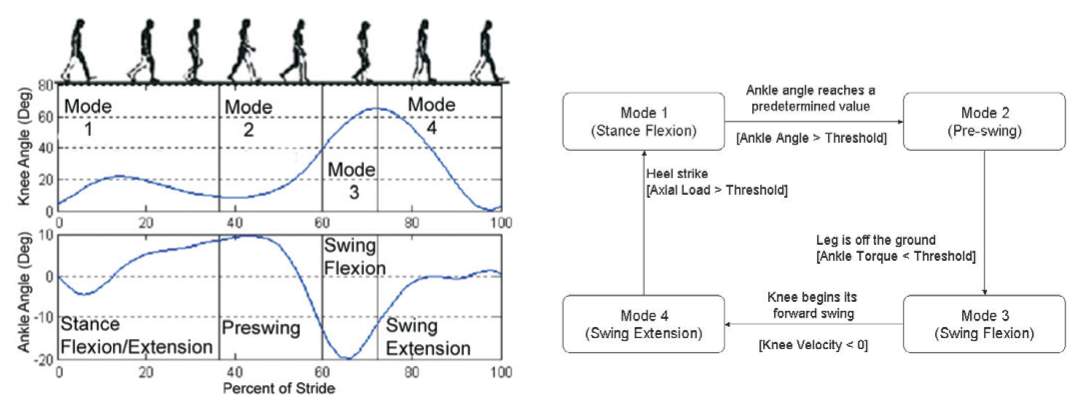
\includegraphics[width=0.95\textwidth]{content/2-Background/state_machine_based_mid_level_controller.pdf}
    \caption[Example state machine for mid level control of a lower limb prosthetic ankle]{Example state machine for mid level control of a lower limb prosthetic ankle \cite{Sup2008b}}
    \label{fig:mid-level-state-machine}
\end{figure}

\subsubsection{Low Level Controller}
The desired device state is passed to the low-level controller. The low-level controller then used closed loop feedback to actuate the prosthetic device. Feedback is based on the error between the current and desired state. There are many forms of controller that are used to achieved this including feed-forward or feedback control.\cite{Tucker2015} Gao et al.~used a Proportional-Derivative controller to regulate the motor current and provide closed loop torque control\cite{Gao2020b}. Yu et al.~used a proportional-integral based closed loop velocity controller to provided velocity control for a hydraulic pump. This was used to regulate the hydraulic pump pressure to drive the hardness and position of a hydraulic actuator.\cite{Yu2019}

%---------------------------------------------%
\section{Sensors}
\label{sec:background-sensors}
To perceive a person's intent, we must take measurements of them\cite{Asif2021, Hernandez2021}. Different sensors allow for different measurements. Each measurement can be of physical quantities about the person or their surrounding environment. Appropriate selection of sensors is therefore of critical importance. Criteria for selection include the type, richness of information and impact on the user.\cite{Tucker2015}

The impact of a sensor considers its invasiveness both physically and in privacy. The physical impact must consider how the discomfort of a sensor affects the performance of an action. For example, a sensor of fewer than 300 grams mounted to a shoe does not affect gait significantly\cite{AbdulRazak2012}. In contrast, many wires rubbing on the leg may. There are also practical concerns, such as ease of use.

Sensing systems divide into three categories: neural, mechanically intrinsic or environmental signals. Neural sensors measure physiological electrical signals, such as brain activity or muscle activity. Mechanically sensors measure effects intrinsic to the device itself, such as acceleration. Environmental sensors measure the properties of the world around them, such as ambient light or pressure.\cite{Koller2018, Tucker2015}

Recent trends in sensing technology have been towards wearable sensors. The demands of the modern smartphone have primarily driven this development. New smaller and more precise sensors have opened up the possibility for making previously lab bound measurements in a more natural environment. Smartphone sensing technology is highly applicable and widely used in active prostheses\cite{Asif2021}; this state of the art review will focus only on wearable technologies.

\subsection{Types of Sensor}
% Mechanical signals
Acceleration and angular velocity are the most commonly mechanically intrinsic signals measured. A wide variety of wearable sensors can collect this information.\cite{Shull2014, Tucker2015} Acceleration and angular velocity are the most commonly mechanically intrinsic signals measured. A wide variety of wearable sensors can collect this information. Other common wearable sensors include goniometer and inclinometers for angular displacements, and pressure transducers or Force Sensitive Resistors (FSR) for foot loading and initial/terminal contact points. Ground Reaction Force (GRF) can also be measured using pressure transducers such as an FSR\cite{Schepers2007}.

The most common wearable sensor used is the \acrfull{imu}\cite{Shull2014}. An \acrshort{imu} is a single integrated circuit containing a three-axis accelerometer and a three-axis gyroscope. The development of smartphones has dramatically reduced the sensors' cost, precision, and size. When an IMU includes a three-axis magnetometer, the sensor becomes a \acrfull{marg} sensor. Using one or multiple sensors allows the determination of limb or joint orientation, angular velocities and accelerations. Figure \ref{fig:bck-imu-sensors} shows a typical IMU sensor and sensor data received from it during different activities from a handheld IMU.

IMUs are widely available, low-cost, and easy to use while giving relatively high accuracy low latency measurements~\cite{Wittmann2019, Bangaru2020}. As they measure physical movement they can be mounted in any location with no dependency on anatomical feature or proximity allowing for very low intrusion measurements\cite{Bangaru2020}. Measurements of an IMUs have physical significance so can be directly interpreted\cite{Godiyal2018a}. IMUs also have low frequency requirements as they measure physical changes of the relatively low frequency human gait cycle. From literature most authors used frequencies around 50Hz\cite{Wang2020, Sabatini2014, Eyobu2018, Su2020, Ordonez2016}.

However, due to the fact that the IMU captures the motion of the forearm, rather than the muscle signal, IMUs sense actions later that neural sensors\cite{Bangaru2020, Godiyal2018a}. IMUs are also sensitive to alignment and placement accuracy. Misalignment results in a change in the axis over which an effect is measured while misplacement can changes the magnitude of accelerations measured\cite{Minor1998}. An IMU also suffers from long term drift and temperature dependent biases\cite{Geiger2008, Minor1998, Wittmann2019}.

\begin{figure}[!hbtp]
    \centering
    \begin{subfigure}[b]{0.45\textwidth}
        \centering
        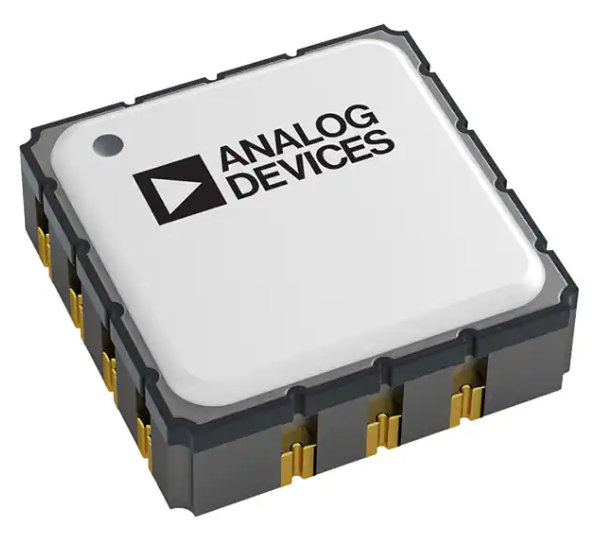
\includegraphics[width=0.7\textwidth]{content/2-Background/sensors/imu_sensor.jpg}
        \caption{Inertial Measurement Unit Sensor\cite{AnalogIMU}}
    \end{subfigure}
    \begin{subfigure}[b]{0.45\textwidth}
        \centering
        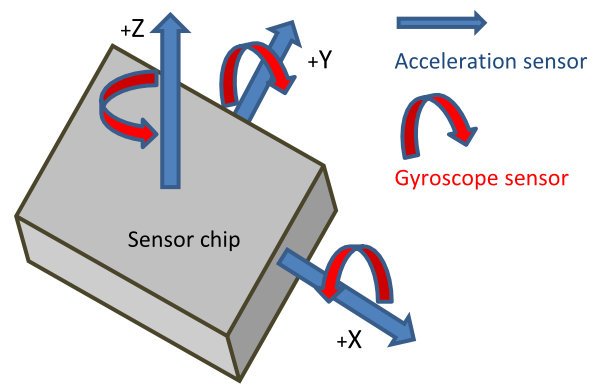
\includegraphics[width=\textwidth]{content/2-Background/sensors/imu_axis.jpg}
        \caption{Inertial Measurement Unit Axis\cite{Kardos2017}}
    \end{subfigure}
    \begin{subfigure}[b]{0.9\textwidth}
        \centering
        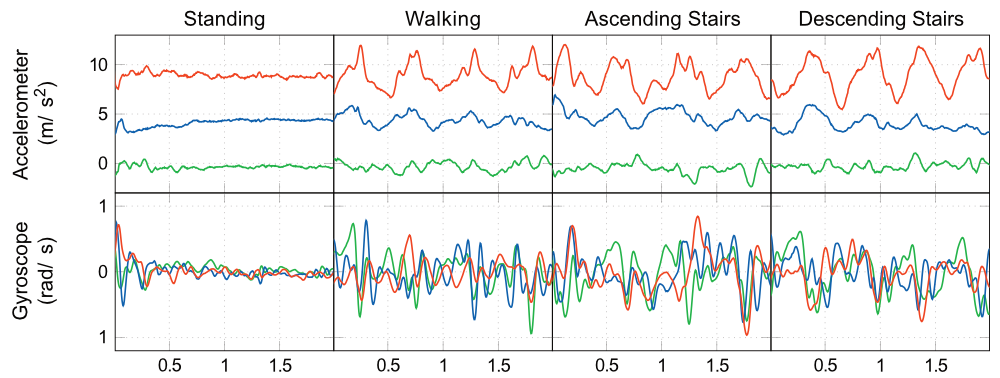
\includegraphics[width=\textwidth]{content/2-Background/sensors/imu_sensor_data.png}
        \caption{Example IMU data\cite{Formento2014}}
    \end{subfigure}
    \caption{IMU sensor and example data}
    \label{fig:bck-imu-sensors}
\end{figure}

\acrlong{fmg} sense volumetric and hardness changes in limbs caused by muscle contraction. Measurements are made by force-sensitive resistors or piezoelectric sensors wrapped around the circumference of the limb. Figure \ref{fig:bck-force-myography-sensors} shows an example thigh worn \acrshort{fmg} sensor and typical sensor data that could be received from it.\cite{Godiyal2018a, Jiang2018}

A potential advantage of \acrshort{fmg} over neural measurements is that the muscle force estimated through \acrshort{fmg} is less sensitive to fatigue. A substantial downside to this approaches is a high sensitivity to motion artefacts, which may be significant given the nature of the physical attachment to the user.\cite{Tucker2015}

\begin{figure}[!hbtp]
    \centering
    \centering
    \begin{subfigure}[b]{0.4\textwidth}
        \centering
        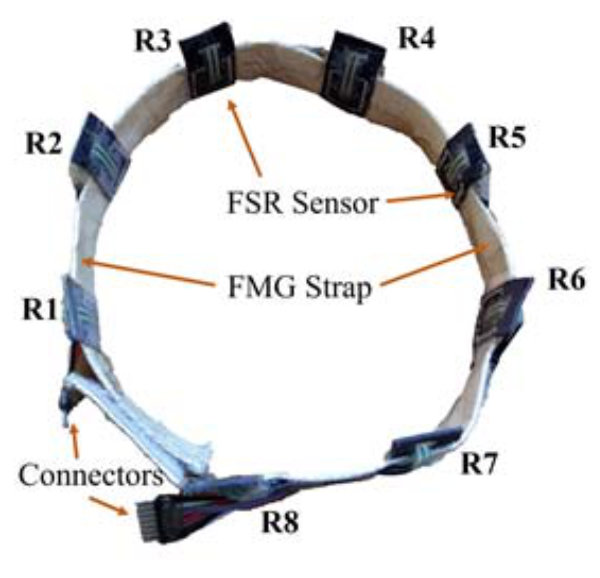
\includegraphics[width=\textwidth]{content/2-Background/sensors/Force-Myography-Sensor.jpg}
        \caption{Force Myography Sensor\cite{Godiyal2018}}
    \end{subfigure}
    \hfill
    \begin{subfigure}[b]{0.55\textwidth}
        \centering
        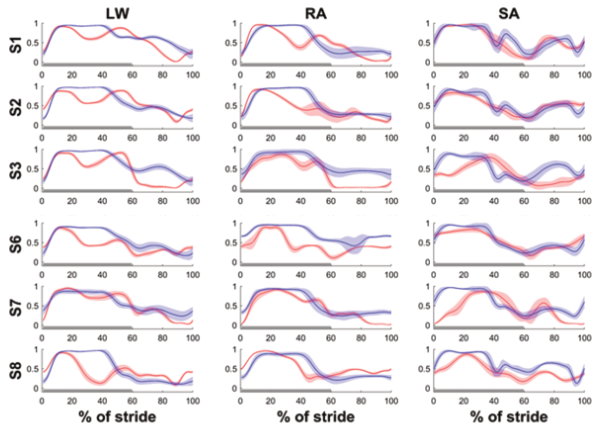
\includegraphics[width=\textwidth]{content/2-Background/sensors/Force_Myography_data.png}
        \caption{Example data\cite{Godiyal2018a}}
    \end{subfigure}
    \caption{Force Myography sensor and example data}
    \label{fig:bck-force-myography-sensors}
\end{figure}

% Neural
Neural signals provide a more natural interface for controlling prosthesis\cite{He2018} but pose significant challenges in there use. Neural sensors detect muscle control signals, where as mechanically intrinsic sensors measure the effect of muscle output. Therefore, neural signals can be detected in order of tens of milliseconds earlier\cite{Tucker2015}, giving longer to perform classification. However, their output is often challenging to interpret due to low signal to noise ratio. Mechanical signals are often more straightforward to measure due to their lower impact and greater tolerance to placement and conditions.\cite{Koller2018} \acrlong{emg} is the most common neural sensor. Electric potential produced by skeletal muscle activity is measured through electrodes attached to the muscle of interest. Figure \ref{fig:bck-emg-sensors} shows an example \acrshort{emg} sensors attached to a trans-tibial amputee's stump and typical data that would be received from it.

% Advantages 
\acrshort{emg} sensors give very early indication of muscle movement as they measure the signals driving muscle movement\cite{Godiyal2018a, Bangaru2020, Huang2011} combined with a very low latency measurement system they can provide a head-start over mechanical sensors\cite{Tucker2015}.
% Disadvantages

However \acrshort{emg} sensors are sensitive to anatomical locations and require skill to fit correctly\cite{Rainoldi2004, Seniam}. They are susceptibility to external factors, such as humidity and movement artefacts\cite{Bangaru2020} and are potentially uncomfortable to wear directly on the skin\cite{Godiyal2018a}. \acrshort{emg} sensors also require high frequency sampling, exceeding 1000Hz, to detect signals sent to the muscle\cite{Huang2011, Young2013}. As the human gait cycle occurs at $0.5$ to $1.3$Hz\cite{Elery2020} this means sensor data must be captured at orders of magnitude above the gait cycle. This high frequency requirement increasing the complexity of capturing and analysing \acrshort{emg} data.

\begin{figure}[!hbt]
    \centering
    \centering
    \begin{subfigure}[b]{0.44\textwidth}
        \centering
        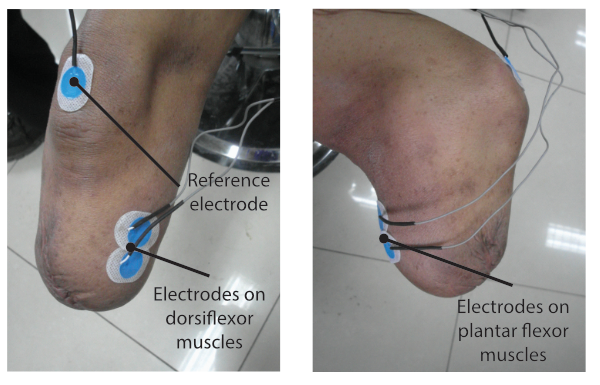
\includegraphics[width=\textwidth]{content/2-Background/sensors/EMG-Amputee_Sensor.png}
        \caption{EMG Sensor\cite{Chen2016}}
    \end{subfigure}
    \hfill
    \begin{subfigure}[b]{0.54\textwidth}
        \centering
        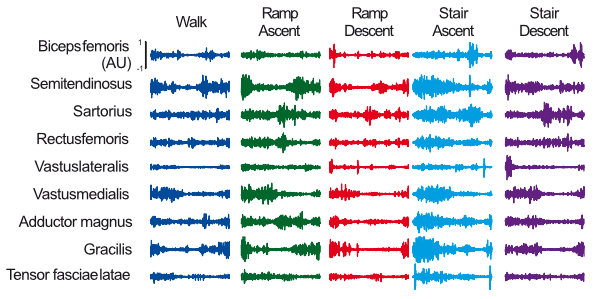
\includegraphics[width=\textwidth]{content/2-Background/sensors/EMG_Sensor_Data.jpg}
        \caption{Example EMG data\cite{Hargrove2015}}
    \end{subfigure}
    \caption{EMG sensor and example data}
    \label{fig:bck-emg-sensors}
\end{figure}

% Environmental
The environment around the user can provide context to local sensor data. Different environments increase the likelihood of encountering a particular terrain feature\cite{Tucker2015, Tschiedel2020}. Care must be taken using environmental sensors as they are highly noisy and susceptible to long term drift. Jin et al.~investigated a evaluated three environmental sensors temperature, humidity, and ambient light. Jin measured repeatable changes in sensor data during different activities. For example during forward motion there was a temperature drop due to airflow over the sensor package.\cite{Jin2014} Figure \ref{fig:bck-temp-sensors} shows a typical temperature sensing integrated circuit and recorded data from a temperature. Fu et al.~investigated the use of a barometric pressure sensor allowing for changes in altitude to be detected\cite{Fu2021}.

\begin{figure}[!hbt]
    \centering
    \centering
    \begin{subfigure}[b]{0.45\textwidth}
        \centering
        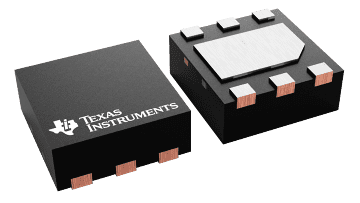
\includegraphics[width=\textwidth]{content/2-Background/sensors/temp_sensor.png}
        \caption{Temperature Sensor\cite{TiTemperatureSensor}}
    \end{subfigure}
    \hfill
    \begin{subfigure}[b]{0.5\textwidth}
        \centering
        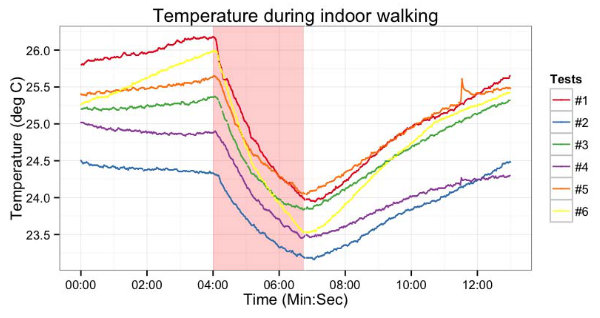
\includegraphics[width=\textwidth]{content/2-Background/sensors/temperature_sensor_data.jpg}
        \caption{Example temperature data\cite{Jin2014}}
    \end{subfigure}
    \caption{IMU sensor and example data}
    \label{fig:bck-temp-sensors}
\end{figure}

% Sensor fusion/multi-modal
Data fusion is research field interested in integrating data from multiple sensors to achieve improved performance\cite{Huang2011}. Sensors can either be multiple of the same sensor\cite{Chung2019} or sensors of different modalities\cite{Huang2011}. Data fusion is regarded as superior to methods that take inputs from a single data source with results indicating fusion methods can increase both accuracy and robustness\cite{Huang2011, Liu2021}.

Chung et al.~used eight \acrshort{imu}s placed across the body. By combining data from multiple sensors performance was improved. Chung also identified that the addition of multiple sensors meant sampling rates as low as 10Hz could be used. \cite{Chung2019}

Liu et al.~and Hu et al.~both combined \acrshort{emg} and \acrshort{imu} sensors. Both found that fused \acrshort{imu} and \acrshort{emg} data gave higher accuracy than with just IMU data.\cite{Hu2021, Liu2021} Huang et al.~fused \acrshort{emg} signals from the thigh with \acrshort{grf} measured from the pylon of a prosthetic devices. The results showed that the fused data outperformed methods that used only \acrshort{emg} signals or mechanical information alone.\cite{Huang2011}


\subsection{Sensor Placement}
The placement of sensors is an important consideration; the chosen location should maximise the richness of data while minimising invasiveness\cite{Tucker2015}.

The prosthetic device is the obvious mounting location providing a rigid and stable sensor platform for prosthetic users. Attachment is more challenging for biological limbs; temporary attachment of sensors by medical tape or elastic strapping is common. Consideration for changing the shape of the limb during movement is required.

Where suitable muscles are present at the skin, electrodes can be attached to the skin's surface above the muscle. Surface EMG presents the least invasive technique for the neural sensory system. However, they must be attached securely to the body to prevent artefacts from corrupting sensor movement readings and require individual calibration.

Shull et al.~reviewed the location of wearable sensors used for gait analysis. Most articles used sensors that are sensitive in the mediolateral axis, with the knee, trunk and shank the most popular sensing location. Figure \ref{fig:shull-sensor-location} shows a visual representation of Shull's findings.

\begin{figure}[!hbt]
    \centering
    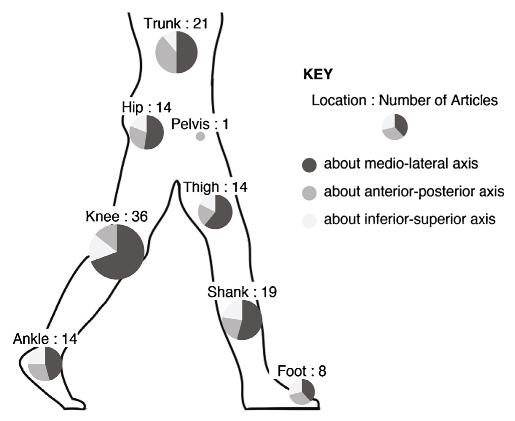
\includegraphics[width=0.6\textwidth]{content/2-Background/shull-2014-sensor-placement.pdf}
    \caption[Target gait parameter locations for wearable sensing]{Target gait parameter locations for wearable sensing. The number of articles reporting gait parameter locations is indicated at each respective location. The diameter of each pie chart is proportional to the number of published articles reporting that gait parameter location. The relative proportion of kinematic and kinetic parameters about each of the three anatomical axes is indicated in the pie charts.}
    \label{fig:shull-sensor-location}
\end{figure}

\acrshort{emg} sensors can be placed in multiple locations however for \acrlong{lmr} the calf and thigh are the most common locations\cite{Xi2019, Li2016, Wang2021a}. There is less consistency for \acrshort{imu}s/ Shin et al.~and Li et al.~both placed sensors on the foot\cite{Shin2021, Li2019a}. Han et al. placed a single IMU directly below the knee joint\cite{Han2021} well Shin et al placed four \acrshort{imu}s on both hips and feet\cite{Shin2021}. There was no obvious improvement in performance from any of the locations.


%---------------------------------------------%
\section{Machine Learning}
\label{sec:background-machine-learning}
% Overview of machine learning aim and operation
\acrfull{ml} is a subset of computer science that focuses on systems that learn from data. An \acrshort{ml} system can numerically estimate a complex function from exposure to examples of a phenomenon. That is to say, an \acrshort{ml} algorithm can convert experience into expertise or make predictions from data. As an entirely numerical approach, it is especially compelling for problems of high dimensionality. There are many different tasks where machine learning can be powerfully used, such as classification, translation, denoising and synthesis.\cite{Mitchell1997, Shalev-Shwartz2014, Goodfellow2015, Burkov2019}

What separates machine learning from optimisation is that we want to minimise the task error not only for the seen experience but also for novel unseen inputs. Minimising the task error forms the crux of machine learning.\cite{Goodfellow2015}

% What is the machine learning process
The machine learning process usually follows three steps; 1) gathering a representative data set; 2) building a model to solve the task based on knowledge captured in the data set; 3) testing and evaluating model performance\cite{Burkov2019}. The output is a model that encapsulates the learnt knowledge. The model is deployable in the real world to perform the taught task.\cite{Shalev-Shwartz2014}.

% How is experience provided
By gathering knowledge from experience, \acrshort{ml} avoids the need to formally specify all knowledge to accomplish a task\cite{Goodfellow2015}. This approach significantly reduces the implementation burden and may enable previously intractable solutions for highly complex systems. Experience is provided as a set or sets of examples of the input and often the corresponding output or label. The set of examples is called the training data.

The model input for each example is a feature vector. Each element of a feature vector contains one quantitative measure of the example. Each feature is either hand picked, such as the mean of a signal, or learnt where raw data is fed directly into the model learnt. The choice of data representation or features can heavily affect the performance of a machine learning system. Hand picking features are labour intensive and without care can result in bias in the machine learning model. However, learnt features require more data for training and are harder to control.\cite{Bengio2013}

The quality of the training data is essential to good learning, as by the adage garbage in, garbage out. However, data quality measurements can be challenging because they must consider qualitative factors such as realism.

The training data is used at various stages throughout the learning process to provide knowledge and verify system performance. The whole training data is split into three sets. Training – a set of examples from which the system learns. Validation – a set used to evaluate the generalisation performance during training. Test – used to evaluate the final generalisation performance after training.

% How is experience converted to knowledge - training/optimisation
Most \acrshort{ml} algorithms involve optimisation of some form. Optimisation refers to the task of either minimising or maximising some function. The function we want to optimise for is called the criterion. The criterion measures what a good prediction is. When minimising the criterion, the criterion is often called the cost or loss function.\cite{Goodfellow2015} The learning algorithm uses the criterion to optimise model weights and biases to incorporate knowledge from the training data.

% Types of training
There are four standard techniques for Machine Learning: supervised, unsupervised, semi-supervised, and reinforcement learning. Each is useful for different tasks and require different forms of experience.

Supervised learning uses a labelled dataset to produce a model that can deduce the correct output from a given input\cite{Burkov2019}. In unsupervised learning, the training data set is unlabelled. The system is left to discover variation and beneficial properties across the data set. Semi-supervised learning lies between supervised and unsupervised. Some but not all example inputs have labels. The algorithm uses known inputs to label unknown examples to build a more extensive labelled training set\cite{Abdallah2018} Reinforcement learning does not experience a fixed dataset. Instead, they interact with an environment using feedback to learn.

% Transfer learning
An additional form of learning is transfer learning. The research field of transfer learning is concerned with the reapplication of captured knowledge. The application changes can be significant, visually identifying a new object, or minor, such as personalisation to an individual. Many schemes exist for achieving knowledge transfer. Schemes include fine-tuning part or all of a model, extending an existing model with additional layers or generating a mapping to adapt a new input source.\cite{Farahani2020, Zhuang2021}

% How is performance measured
Understanding the final performance of the trained model requires additional metrics as the loss function is often not directly interpretable. These quantitative metrics represent the \acrshort{ml} system's ability to perform the desired task. Often the metric will be directly inheritable, such as the proportion of examples where the output was correct. The performance metric is generally evaluated for all three data sets to evaluate different aspects of model performance. For example, generalisation, or the performance for unseen data, can be evaluated using the test set.

% Other aspects of machine
Many issues may occur while developing an \acrshort{ml} system. For example, over/under-fitting. Fitting problems occur when the model either learns too tightly to the training set or cannot learn the desired task. Therefore it cannot predict new unseen inputs. Adjustments to the learning rate, training data or training time will affect fitting. Adjustments to system hyper-parameters control properties such as these. Any settings determined outside the learning algorithm are called hyper-parameters.\cite{Goodfellow2015}

% How are machine learning models constructed
Many \acrshort{ml} models exist and have been used widely across many different tasks. Some typical machine learning models are Random Forest, \acrfull{svm}, \acrfull{mlp} (Dense when fully connected), \acrfull{cnn}, \acrfull{rnn}.

\acrshort{mlp}, \acrshort{cnn} and \acrshort{rnn} are all forms of \acrfull{ann}. They are referred to as networks because they are typically implemented by composing together many different functions. The neural aspect comes from the original inspired by replicating biological neurons.

Multiple layers of neuron units form an \acrshort{ann}. The layer location in the neural network determines its name. The first network layer that receives input data is called the input layer. The network's last layer is called the output layer for similar reasons. The intermediate layers are hidden layers. By adding more layers and more units within each layer, a network can represent functions of increasing complexity\cite{Goodfellow2015}.

Each layer in a neural network is composed of many cells or units. The cell's make-up depends on the type of layer. The connections between cells are also dependent on the layer type. All cells have at least one feed-forward connection to the next layer. A fully connected layer is where each cell connects to every cell on the next layer. When forward feed networks include feedback connections, they are called \acrshort{rnn}s.

Two common ML architectures are \acrshort{cnn}s and \acrshort{rnn}s. The CNN is a specialised neural network that use convolution to combine inputs. They are well suited to grid-like data such as images or regular sampled time-series data. This architecture has been successful in practical applications, primarily visual problems.\cite{Goodfellow2015}

%-------------------------------------------------------------------
\section{Long Short Term Memory (LSTM)}
The RNN is a family of neural networks widely used in the field of translation, text, and time series prediction. There structure allows them to process longer sequences than practical for other networks.\cite{Goodfellow2015} They are superior to a standard \acrshort{rnn} system as they overcome well-documented issues such as the ``vanishing gradients'' problem. Vanishing gradients arise from the large chain of multiplication that occurs when performance error back propagation in an \acrshort{rnn}.\cite{Sherstinsky2020, Lee2021}

% RNN unfolding/unrolling\cite{Sherstinsky2020}

The LSTM resolves some of the issues with vanishing gradients by introducing gates to controls information flow\cite{Hochreiter1997}. During training the gates learn to forget thus to regulating information held\cite{Hernandez2021}. Since conception \acrshort{lstm}s have become popular with many researchers as an effective and scalable model for learning problems related to sequential data.\cite{Greff2017, Yu2019} There are still issues that must be considered, such as a tendency for the output to converge based on a straight pattern since the input order is chronological.\cite{Lee2021}

The original \acrshort{lstm} cell was created by Hochreiter and Schmidhuber in 1997~\cite{Hochreiter1997} but has been improved upon by multiple researchers. The most common form used today features the forget gate introduced by Gers et al.\cite{Gers2000, Yu2019}. The Gers's cell architecture is shown in Figure \ref{fig:bck-lst-architecture}.

\begin{figure}[!htb]
    \centering
    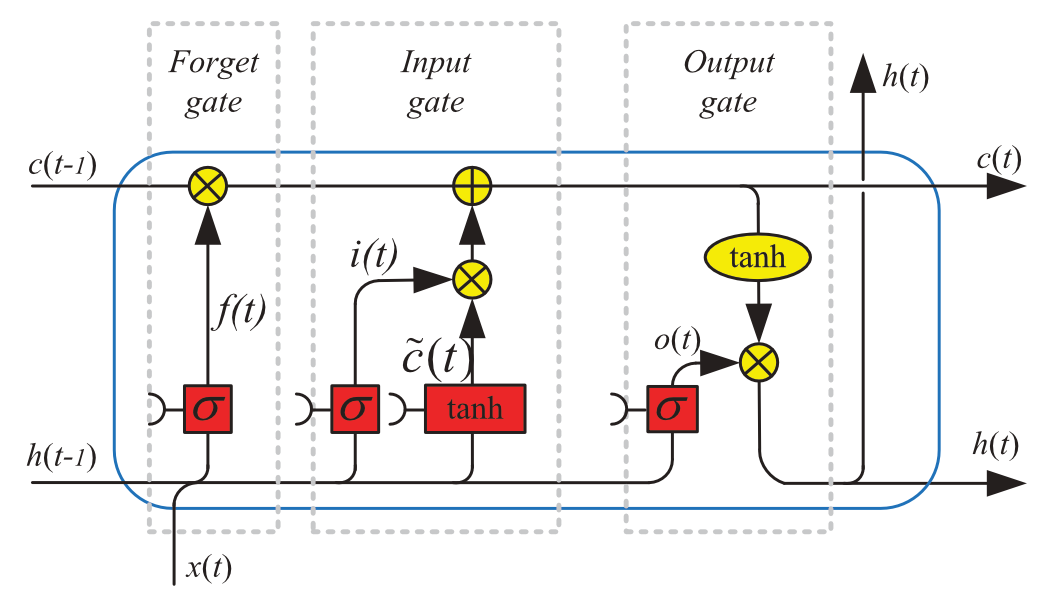
\includegraphics[width=0.8\textwidth]{content/2-Background/lstm_with_forget_gait.png}
    \caption[LSTM with Forget Gate]{LSTM with Forget Gate\cite{Yu2019}}
    \label{fig:bck-lst-architecture}
\end{figure}

An LSTM cell learns to add or removing information to the cell state, $c(t)$. This cell state is regulated using the forget $f(t)$ and input $i(t)$ gates. The forget gate determines what information to forget, while the input gate determines whether new information should be added to the cell state. So the new cell state is a function of the previous cell state ($c(t-1)$), modulated by the current input ($x(t)$) and the previous hidden state ($h(t-1)$), combined with some of the current input ($x(t)$). The output from the \acrshort{lstm}, termed the hidden state $h(t)$, is a function of the new cell state modulated by the output gate ($o(t)$).\cite{Lee2021}


%---------------------------------------------%
\section{Locomotion Mode Recognition}
\label{sec:background-ml-lmr}
Classifying human activities from sensor data is challenging. The signal difference between activities is often subtle and highly individualised.\cite{Zhu2019} Many different methods have been tested to address this problem including heuristic, statistical and machine learning methods.

%---------------------------------------------%
\subsection{Non-ML Methods}
There are numerous forms of activity classifiers that do no use machine learning techniques. These include manual rule based heuristic methods and pattern recognition.

These have the advantage of usually being simpler both in operation and also understanding than machine learning methods. However, they normally require manual tuning and setup to adapt to an individual and struggle with higher dimensional data\cite{Tucker2015}. As well, the classification output can only be made after the rule has been completed so there is a delay in outputting a classification.

A activity recognition heuristic is usually a fixed set of rules that controls the transition between activity modes. Heuristic methods are the current standard for modes selection in powered prostheses\cite{Varol2008, Lawson2014, Gorsic2014, Young2014a}. However there are very limited contemporary reference of these methods being used.

Formento el al.~presented a heuristic for classifying walking, stair ascent and descent based on the output from a gyroscope. It was established by coley et \cite{Coley2005} that the sagittal plane output of a shank mounted gyroscope varies during stance depending on the activity. Detection success was over 93\% however the classification can only be made after the step has occurred. Figure \ref{fig:bck-stair-heuristic} shows an illustration of the heuristic.\cite{Formento2014}

\begin{figure}[!htb]
    \centering
    \begin{subfigure}[b]{0.54\textwidth}
        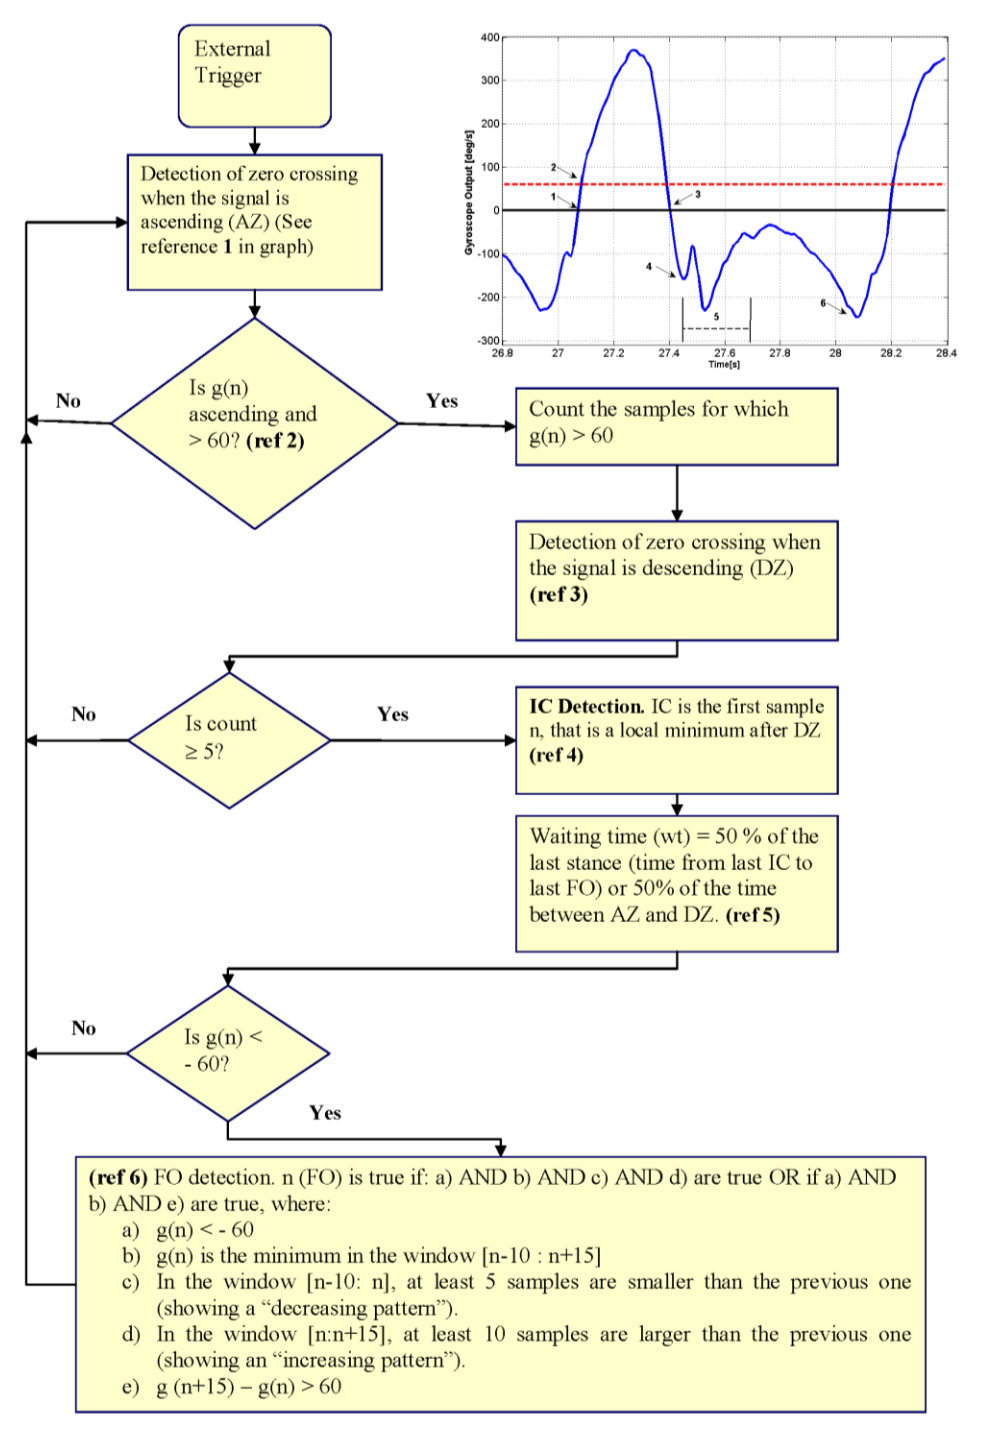
\includegraphics[width=\textwidth]{content/2-Background/stair_heursitic.jpg}
        \caption{Heuristic rules \cite{Formento2014}}
    \end{subfigure}
    \begin{subfigure}[b]{0.28\textwidth}
        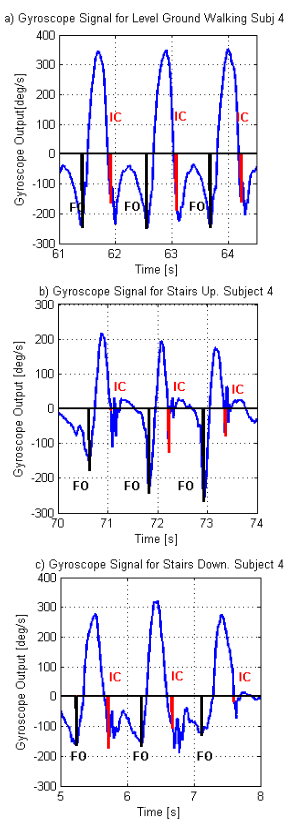
\includegraphics[width=\textwidth]{content/2-Background/stair_gyro_signals_2.png}
        \caption{Example input data \cite{Formento2014}}
    \end{subfigure}
    \caption{Stair Ascent and Descent Heuristic}
    \label{fig:bck-stair-heuristic}
\end{figure}


%----------------------------------------------------------------------------
\subsection{Machine Learning Methods}
% How can machine learning be useful for activity recognition
Researchers have produced many machine learning architectures for solving \acrshort{har} problems\cite{Wang2019b}. Typically, \acrshort{har} \acrshort{ml} models all follow the same structure. A window of sensor data is collected and fed directly into the model. This direct approach improves the signal-to-noise ratio\cite{Hernandez2021}. The model classifies the activity producing the corresponding output. Figure \ref{fig:back-sensor-based-deep-learning} illustrates this structure.\cite{Wang2019b}

\begin{figure}
    \centering
    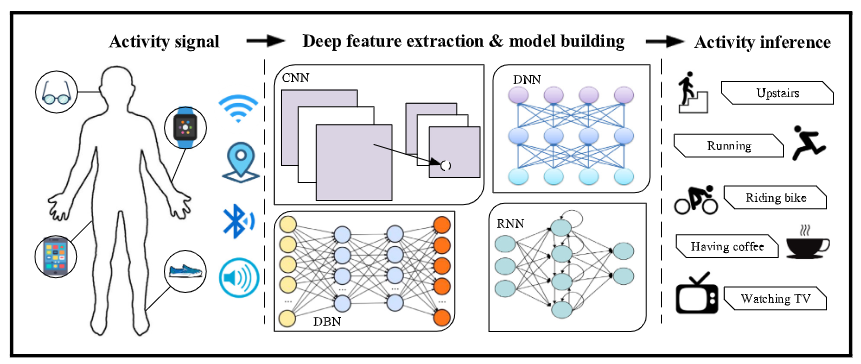
\includegraphics[width=0.9\textwidth]{content/2-Background/sensor-based-deep-learning.png}
    \caption[An illustration of sensor-based machine learning activity recognition]{An illustration of sensor-based activity recognition using a machine learning approach\cite{Wang2019b}.}
    \label{fig:back-sensor-based-deep-learning}
\end{figure}

Machine learning methods offer the potential to achieve higher performance, for more classes, with less manual input\cite{Hernandez2021, Zhu2019, Rai2019}. Deep learning can also provide increased flexibility, robustness and improved performance. However their learning can be difficult to control, and the solution difficult to understand\cite{Edwards2018, Greff2017}. \acrshort{ml} systems also require a large amount of data to train\cite{Nguyen2021a}. For target users whose behaviour differs significantly from the training dataset the user may suffer degraded performance. It can also be extremely laborious or impractical to collect and label large set of data, especially for the elderly and disabled people.\cite{Qiu2022}

% Types of machine learning models
Most researchers developing machine learning processes for \acrshort{har} use a supervised learning approach\cite{Saini2020, Straczkiewicz2021}, with only a few examples of unsupervised and semi-supervised learning\cite{Bota2019}.

Locomotive data is usually continuous time series in nature. The continuous sensor data must be split and labelled with the current activity for supervised learning methods. The most common form of this is to use a sliding window that divides continuous data into chunks. The activities encompassed by the window determine its label.

A large number of papers use \acrfull{cnn} and \acrfull{lstm} networks to implement \acrshort{har}. Both network types are well suited to regularly sampled sensor data.

\acrshort{cnn} architectures use convolutional and pooling layers to extract features from the sensor data. A dense \acrshort{mlp} layer forms the final classification based on the outputs from the final \acrshort{cnn} layer.\cite{Jiang2015, Lu2020, Martinez-Hernandez2021}

\acrshort{rnn} networks have been used frequently for \acrshort{har} problems. The most commonly implementation uses \acrshort{lstm} cells. The layer structure of \acrshort{lstm} networks is such that the output of each \acrshort{lstm} unit layer is fed only into the \acrshort{lstm} units at the same time step. The formation of final classification uses either all the outputs of the last layer or only the last set of units.\cite{Yu2018, Uddin2021a}

Recently researchers have begun combining \acrshort{cnn} and \acrshort{lstm} networks to form Deep Convolutional and \acrshort{lstm} networks\cite{Ordonez2016}. The convolutional layers are placed either as the input or just before the output.\cite{Mutegeki2020, Xia2020}

Both \acrshort{lstm} and \acrshort{cnn} networks are used extensively throughout literature, Performance for these networks is high with most achieving >95\% accuracy on publicly available data sets collected in lab conditions. Data from \acrshort{imu} sensors is the most common input into these networks.\cite{Murad2017, Su2019, Tufek2020, Xia2020,  Ma2021, Uddin2021a}

%----------------------------------------------------------------------------
\subsection{Personalisation Techniques}
\label{sec:personalisation-related-works}
\acrshort{ml} classifiers are constructed assuming that the probabilistic distribution between the source and target domain are equal\cite{Farahani2020}. In reality, this is never the case, so methods to account for differences between domains have been developed. Where the model is adapted to an individual user, this is typically termed personalisation.

Personalising \acrshort{ml} models is a common issue and has been addressed in many ways across different research areas\cite{Mairittha2021, Tomanek2021}. Schneider et al.~divide personalisation methods into two groups, shaping and data grouping\cite{Schneider2021}. In shaping the behaviour of a network is biased or shaped towards an individual, in data grouping, the target data set is enlarged by adding data from similar individuals to it. Both of these techniques take advantage of data from others to reduce labelled data requirements for the target subject\cite{Shor2020}. The following survey of literature will be divided into these two categories.

Shaping the behaviour of a network can occur at different times during training. Two are common, the beginning, early, or the end, late. In early shaping, the model is first trained with target data, followed by a more extensive source data set. The opposite is done in late shaping, where a general model formed from a large source training set is fine-tuned with target data. Fine tuning is performed by additional training of a pre-trained model with a different training set. This method is common and generally referred to as transfer learning.\cite{Schneider2021}

Transfer learning is the ability to extend what has been learnt in one context to another non-identical but similar context\cite{Fallahzadeh2017}. The change in context can be either the task, the domain or both. Transfer learning is appealing since it is often faster, as a model does not need to be trained from scratch for each target.

Transfer learning is generally achieved in two phases. First, a generic global model is trained from a source data set. Then it is adapted to the target by additional training using only the targets data. The influence of the target is controllable by both the number of iterations and the number of layers trained.\cite{Schneider2021, Mireshghallah2021}

A subset of transfer learning is domain adaptation, where the domain changes but the task remain the same\cite{Goodfellow2015}. Domain adaptation techniques often focus on learning and applying a mapping between the source and target input data rather than fine-tuning an existing model.

%-----------------------------
% Shaping/Transfer learning
Yoon et al.~presented a transfer learning scheme for personalising an \acrshort{lstm} based language model trained to generate stylised sentence completion. Their work focuses on techniques that allow transfer learning using only a small quantity of target data and limited computing resources. Two schemes are investigated to achieve this reduction: training a new layer between the output and last \acrshort{lstm} layer, and freezing the first n-layer and fine-tuning just the subsequent layers. Both methods reduce the training requirements compared to fine-tuning the entire base model while achieving similar performance.\cite{Yoon2017}

Fu et al.~developed a domain adaptation method for unlabelled target data denoted Joint Probability Domain Adaptation with Improved Pseudo Labels (IPL-JPDA). The method produces a transformation matrix to adapt the input data of the target to the source domain removing the need to adjust the model itself. The study collects labelled data for a set of ten subjects in a controlled environment. This data is then split into target and source data sets with the performance tested using a cross-validation method. Personalisation is undertaken using the IPL-JPDA method and tested against a subset of the data windows for each activity. Their method achieves $93.2\%$ accuracy, an increase of around $2\%$ over the baseline.\cite{Fu2021}


%-----------------------------
% Data grouping - Training from similar users
The other category of personalisation is data grouping. In data grouping, the target data set is enlarged by supplementing it with data from existing source data. Each individual will differ from others, but it should be expected that the population as a whole or a subset of it are similar\cite{Schneider2021, Nguyen2021}. Identifying and combining similar individuals is the central area of concentration for this field.

Ferrari et al.~investigated data grouping personalisation methods that weight the influence of training data based on similarity to the target subject. Individual's similarity was evaluated by comparing physical traits (age, weight and height) and input feature vectors. Three public \acrfull{adl} data sets were used to test performance, niMiB-SHAR\cite{Micucci2017}, Mobiact\cite{Vavoulas2016} and Motion Sense\cite{Katevas2014}. All data sets were collected in controlled conditions. Using the weighted training data, an Adaboost classifier was trained for each target subject. The experiment was repeated with and without target data included in the training set. Excluding the target saw only a small performance improvement, compared to without similarity biasing. Including the target in the training data increased classification accuracy by $>10\%$, on average achieving $87.39\%$. These results suggest that weighting the training data set towards the target subject has a larger influence on performance than similarity on its own.\cite{Ferrari2020}

Nguyen et al.~presented another data grouping technique using a DeepConvLSTM architecture. The model used learnt features, so determining the similarity of the feature vector was not possible. Instead, the output of the last LSTM layer was used as a pseudo for the feature vector. A \acrfull{fid} algorithm was used to score the similarity of subjects. The score was then used to group source subjects by two schemes: selecting the closest $n$ neighbours and clustering subjects into communities. It was noted that this correlated closely with physical characteristics. The groups were then used to train a new model from scratch and fine-tune a general model. Fine-tuning a global model proved more effective. This method improved the global model performance by $3.5\%$ to $84.2\%$. The experiments were performed on four public data sets; OPPORTUNITY\cite{Roggen2009}, Daphnet Gait\cite{Sigcha2020}, Wetlab\cite{Scholl2015} and Mobiact\cite{Vavoulas2016} data sets, all of which were collected in closed controlled environments.\cite{Nguyen2021}

%-----------------------------
% Combination - retrain general model based on similar users
Several authors attempted to combine both transfer learning and data grouping techniques. These methods used data grouping techniques to produce a base model, which was subsequently fine-tuned using data from the target.

Wang et al.~presents a source selection and transfer learning approach for a \acrshort{cnn}-\acrshort{lstm} architecture for unsupervised transfer learning. First source subjects were selected based on a closeness score. This score combined a cosine similarity function and a hand-selected value based on the physical similarity between sensor locations. Using the selected source subjects an \acrshort{ml} model was trained. Fine-tuning of the model was achieved by inserting and training an adaption layer between the last two dense layers. The investigation was performed using the OPPORTUNITY\cite{Roggen2009}, PAMAP2\cite{Reiss2012} and UCI DSADS\cite{Altun2010} data sets, which again were all collected in controlled conditions.\cite{Wang2018a}

Cruciani et al.~presented work on personalising an activity recognition model built from the subset of a general population. The subset of subjects was selected by comparing the similarity of manually selected features. Those with the closest matching traits were used to generate the base model. Further training was then performed using a small amount of target data. This approach achieved a ~5\% improvement in performance when compared to selecting a source subset at random\cite{Cruciani2020}. The experiment was performed on the \acrshort{adl} Extrasensory data set published by Vaizman et al.\cite{Vaizman2017}, this data set was collected using a smartphone in uncontrolled conditions with limited guidance given on how to collect or label the data.


%----------------------------------------------------------------------------
\subsection{Application to Amputees}
% How is this useful for amputees?
The gait of a lower-limb amputee varies dramatically between individuals\cite{Lonini2016} often presenting asymmetrically\cite{Roerdink2012}. This asymmetry results in a substantially different gait from the norm. Therefore techniques that work for non-amputees are not necessarily directly applicable to amputees or other gait impairments\cite{Jamieson2021}. As \acrshort{ml} performance degrades where a similar user is not in the training pool personalisation of a model is really important for amputees.

Bespoke models can achieve good classification performance for individuals, including amputees. However, there is still significant room for improvement of \acrshort{imu}-based LMR classifiers. The difficulty in collecting amputees' data limits research in this area and the practicality of deploying a developed system. Therefore any system that can leverage knowledge from other more obtainable sources would be highly advantageous. None of the three studies into amputees have publicly released their data.

Only a few papers have applied \acrshort{ml} techniques to the problem of \acrshort{imu}-based \acrshort{lmr} classifiers for amputees. Of them, only three papers have tested their methods on amputee gait data\cite{Lu2020, Bruinsma2021, Jamieson2021}. The lack of testing on amputees is likely due to the difficulties of collecting gait data from amputees\cite{Gardiner2016}.

Bruinsma et al.~tested different configurations of \acrshort{rnn} and \acrshort{cnn} networks. Gait data from a trans-femoral amputee was collected. The amputee wore two \acrshort{imu}s mounted on the thigh and shank. All collection of gait data was in a controlled environment. The gait data did not include any non-amputees subjects for comparison. Evaluation of different network architectures revealed that the \acrfull{gru} and \acrshort{lstm} networks performed highest, achieving greater than 80\% accuracy. The best performance of  93.06\% occurred when using a \acrshort{gru} network fed with data from both \acrshort{imu}s.\cite{Bruinsma2021}

Su et al.~demonstrated \acrshort{cnn} classifiers with both amputees and non-amputees. Su produced an \acrshort{imu} dataset collected in a controlled environment to test the classifiers. Ten non-amputee and a single trans-tibial amputee were asked to walk up and down a single staircase, ramp, and flats. The \acrshort{imu} was placed on the healthy leg of the amputee. Both a general classifier tested with a subject not used for training and a bespoke classifier trained and tested with data from a single individual were tested. The bespoke classifier performed as highly, achieving an average performance of $94\%$ for the ten non-amputees and $89\%$ for the single trans-tibial amputee. The results of the general model showed a drop in performance to an average of $82\%$. It is not clear if this number includes performance using the trans-tibial amputee.\cite{Su2019}

Jamieson et al.~performed a study comparing the performance of supervised classifiers for both amputee and non-amputee carrying out the same activities. Jamieson collected a dataset of \acrshort{imu} gait data from eight non-amputees and four subjects with lower limb amputation. Each subject wore a single hip worn \acrshort{imu} as they walked an improvised route through a natural environment.e in the vicinity of their homes.  Both \acrfull{svm} and \acrshort{lstm} networks were trained to classify different locomotive activities. Classifiers were trained with varying sets of data constructed by \acrfull{looxv}. Several configurations of subjects were tested. Most notably, a network was trained using exclusively non-amputee data but tested using amputees. Classification accuracy fell from $~78\%$ for non-amputees to an average of $~28\%$ for the four amputees. Jamieson concluded that classifiers trained using exclusively persons without gait impairments would not be suitable for impaired gait.\cite{Jamieson2021}

Lonini et al.~considered a personal model trained from a target's data to be required; or alternatively, a global model trained from other similar patients. The study involved classifying physical activities based on sensor data from a waist-worn accelerometer. Eleven non-amputee and ten patients who use a Knee-Ankle-Foot Orthotic (KAFO) device were asked to perform five actions. Their work suggested that models trained exclusively from subjects without gait impairments perform poorly when tested using the KAFO subjects. However, the model trained from only KAFO subjects performed slightly worse than a baseline personalised model.\cite{Lonini2016}

Gao et al.~presented work investigating Reinforcement Learning (RL) schemes for controlling a lower limb prosthesis personalised to an individual. They first collected data from two non-amputees wearing a below-knee prosthetic device. This data was used to generate base knowledge that could be used as a starting point for their RL scheme. Using the human locomotive simulator OpenSim they implemented models of amputee gaits. These were then used to demonstrate an RL scheme that could adapt to an individual.\cite{Gao2020a}

There is limited literature on applying classifiers built from non-amputee data to amputees or those with other gait abnormalities. However, literature suggests that in order to achieve adequate classification accuracy gait abnormalities of an amputee must be taken into account.

%---------------------------------------------%
\section{Conclusions}
\label{sec:background-conclusion}
Gait is a highly individual trait. The human body has evolved to use distinct control modes for accomplishing different locomotive actions. Lower limb amputees have many gait difficulties. For a lower limb prosthetic device to fully restore the lost functionality, it must be powered and replicate the different control modes. Part of the challenge of achieving this is determining the locomotive intent of a subject.

Machine learning has made significant inroads in identifying human activities from low-cost \acrshort{imu}s likely to be present on powered lower limb prostheses. However, limited research has occurred in machine learning techniques for human activity recognition of lower limb amputees. The lack of research is likely due to the difficulties of collecting gait data from amputees. Research into ways to reduce the data requirements for \acrshort{imu}-based locomotion mode recognition systems for lower limb prosthesis is required.
